\subsection{Termux}
\begin{enumerate}[label=\arabic*.,ref=\theenumi]
	\item On your android device, follow the instructions in 
%fdroid apk from
%
\begin{lstlisting}
https://github.com/gadepall/fwc-1
\end{lstlisting}
to setup and install Debian on Termux.
\iffalse
\item Install Termux from apkpure
\item Install basic packages on termux 
\begin{lstlisting}
#Give termux access to your  user directory in android
termux-setup-storage

#Upgrade packages
apt update && apt upgrade
apt install build-essential openssh

#Mandatory packages
apt install curl git wget subversion proot proot-distro python  nmap neovim ranger
#------------------End Install Termux----------------------------
\end{lstlisting}
\item Install debian on termux 
\begin{lstlisting}
proot-distro install debian
proot-distro login debian
\end{lstlisting}
\fi
\end{enumerate}
\subsection{Platformio }
\begin{enumerate}[label=\arabic*.,ref=\theenumi]
	\item Install Packages
\begin{lstlisting}
apt install avra avrdude gcc-avr avr-libc
\end{lstlisting}
\item Follow the instructions in 
\begin{lstlisting}
https://docs.platformio.org/en/stable/core/installation/methods/installer-script.html#super-quick-macos-linux
\end{lstlisting}
to install platformio.
\item Execute the following on debian
\begin{lstlisting}
cd ide/piosetup/codes
pio run
\end{lstlisting}
\item Connect your arduino to the  laptop/rpi and type
\begin{lstlisting}
pio run -t nobuild -t upload
\end{lstlisting}
\item The LED beside pin 13 will start
	blinking.  See \figref{fig:arduino} for the Arduino pin diagram.
		\begin{figure}[H]
	\centering
	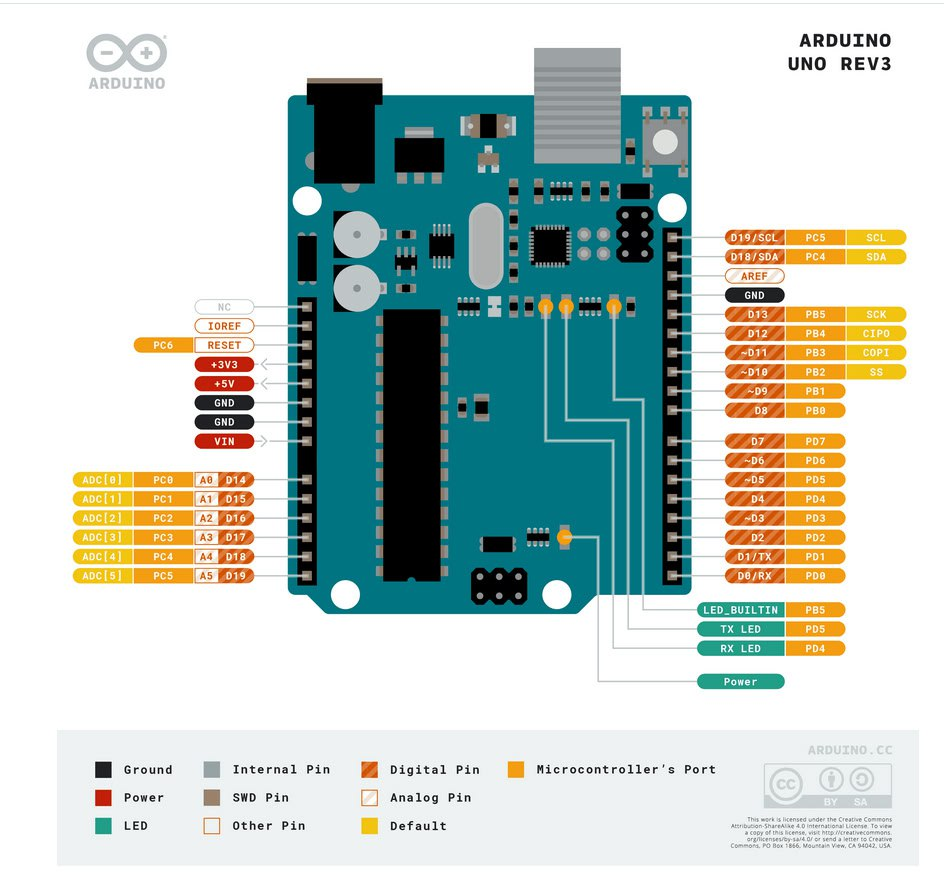
\includegraphics[width=0.75\columnwidth]{figs/arduino.jpg}
	\caption{}
	\label{fig:arduino}
\end{figure}

\end{enumerate}
\subsection{Arduino Droid}
\begin{enumerate}[label=\arabic*.,ref=\theenumi]
\item Install ArduinoDroid from apkpure
\item Open ArduinoDroid and grant all permissions
\item Connect the Arduino to your phone via USB-OTG
\item For flashing the bin files, in ArduinoDroid,
\begin{lstlisting}
Actions->Upload->Upload Precompiled
\end{lstlisting}
then go to your working directory and select
\begin{lstlisting}
.pio/build/uno/firmware.hex
\end{lstlisting}
for uploading hex file to the Arduino Uno
\item The LED beside pin 13 will start
blinking
\end{enumerate}




